\subsection{实验设计}
本实验围绕向量求和程序的性能优化展开，目标是在保证计算结果正确的前提下，比较不同优化方法对程序执行效率的影响。根据实验要求，本任务需要在香山仿真环境中对示例代码进行实现、优化与性能分析，并通过性能指标评价优化效果。实验中统一采用长度为10000的整型向量作为输入，使用 \texttt{CSR\_MCYCLE} 记录核心求和函数的执行周期数，作为主要性能评价指标。

本实验共设计了6个版本的向量求和程序，其中包括1个基线版本、4个手工代码优化版本和1个编译器优化尝试版本。各版本的设计思路如表所示：

\begin{table}[H]
\centering
\caption{向量求和优化版本迭代说明}
\begin{tabular}{lll}
\toprule
版本分类 & 核心技术 & 优化逻辑说明 \\
\midrule
基线版本 & 原始逐元素求和 & 使用 \texttt{vec\_length()} 与 \texttt{get\_vec\_element()} 完成循环读取与累加，结构清晰但过程调用开销较大 \\
优化一 & 直接数组访问 + 局部累加 & 去除不必要的过程调用，直接访问 \texttt{v->data}，并使用局部变量累加后统一写回 \\
优化二 & 4路循环展开 & 每轮循环同时处理4个元素，并设置4个独立累加器，减少循环控制开销和顺序相关 \\
优化三 & 指针遍历 + 4路展开 & 在优化二基础上改用指针遍历，希望减少地址计算开销 \\
优化四 & 8路累加器 + 8路展开 & 进一步扩大循环展开规模，利用更多独立累加器增强指令级并行性 \\
编译器优化尝试 & 函数级 \texttt{O3} & 在优化四基础上增加 \texttt{\_\_attribute\_\_((optimize("O3")))}，考察编译器优化的额外作用 \\
\bottomrule
\end{tabular}
\end{table}

\subsection{实验过程}
首先，按照实验文档附录3完成香山仿真环境的配置与验证工作。具体包括克隆 \texttt{xs-env} 仓库，执行 \texttt{setup-tools.sh} 安装依赖，使用 \texttt{source setup.sh} 和 \texttt{source env.sh} 配置环境变量，并检查相关路径是否正确加载。之后进入 \texttt{nexus-am/apps/hello} 目录，将实验代码放入 \texttt{hello.c} 中，通过 \texttt{make ARCH=riscv64-xs} 进行编译，生成对应的 \texttt{.elf}、\texttt{.bin} 和反汇编文件；再进入 \texttt{NEMU} 目录，使用 \texttt{riscv64-nemu-interpreter} 加载生成的二进制镜像进行运行。通过这一过程，验证了任务二代码能够在香山仿真环境中被正确编译和执行，为后续优化实验奠定了基础。

在确认程序能够正常运行后，首先测试基线版本。基线版本采用最原始的向量求和实现方式，在循环中通过 \texttt{vec\_length(v)} 获取向量长度，并通过 \texttt{get\_vec\_element()} 获取每一个元素，然后再逐项累加到结果变量中。该写法逻辑清晰，便于验证程序正确性，但存在明显的函数调用、边界检查和频繁存储访问开销，因此将其作为后续所有优化版本的参照标准。实验结果表明，基线版本能够正确输出向量和 \texttt{50005000}，并测得核心求和函数的周期数为 \texttt{50012}。

下面给出基线版本运行结果截图，用于说明原始版本程序能够正确执行，并为后续优化提供初始性能基准。

\begin{figure}[H]
    \centering
    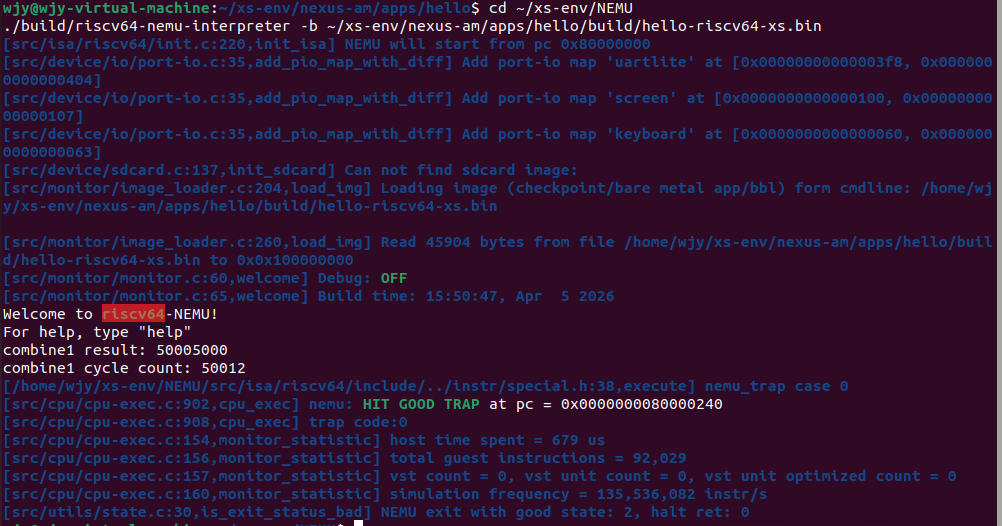
\includegraphics[width = 1\textwidth]{figure/original.png}
    \caption{任务二原始版本运行结果截图}
\end{figure}

在得到基线结果后，开始依次进行多轮手工代码优化。

第一轮优化的核心思想是减少不必要的过程调用，直接使用 \texttt{v->len} 和 \texttt{v->data} 访问向量长度和数组内容，并使用局部变量完成累加后再统一写回结果。这样可以有效减少循环体中的函数调用与中间访存开销。
\begin{figure}[H]
    \centering
    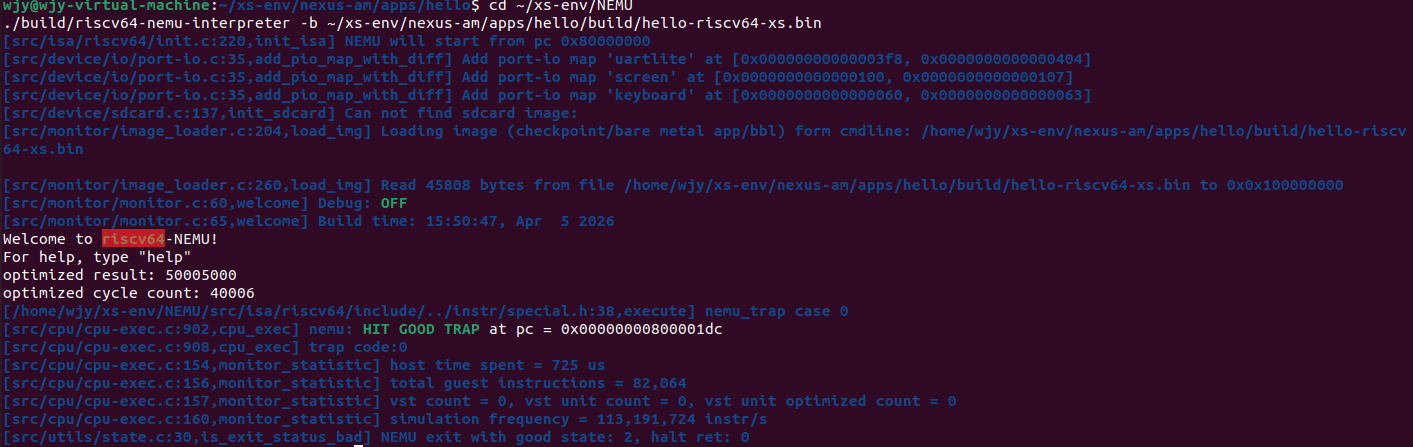
\includegraphics[width = 1\textwidth]{figure/one.png}
    \caption{任务二优化一运行结果截图}
\end{figure}
第二轮优化在此基础上引入 4 路循环展开，使每轮循环同时处理 4 个元素，并使用多个独立累加器减轻顺序相关带来的性能限制。实验结果显示，优化二的周期数明显下降，说明循环展开在当前实验环境下具有显著效果。
\begin{figure}[H]
    \centering
    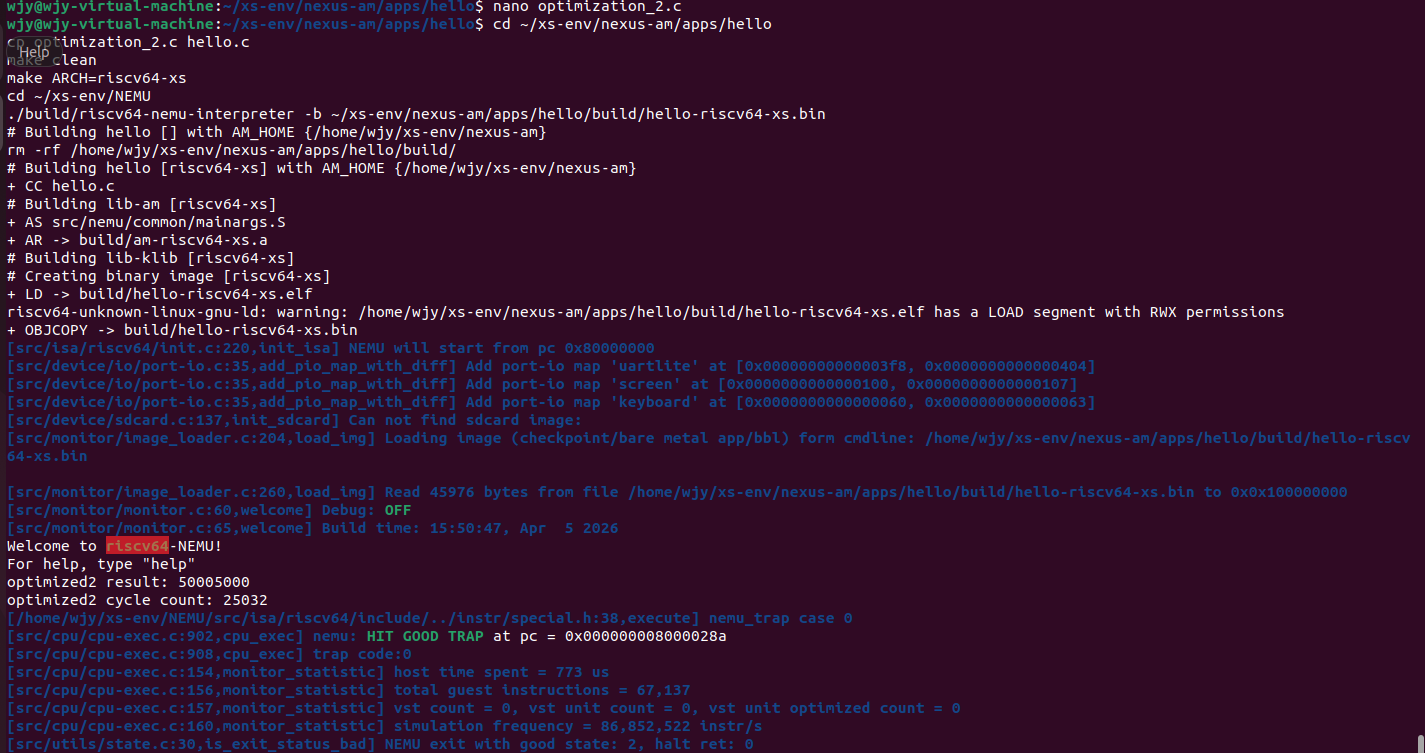
\includegraphics[width = 1\textwidth]{figure/two.png}
    \caption{任务二优化二运行结果截图}
\end{figure}
在优化二之后，又继续尝试优化三和优化四。

优化三在优化二基础上改用指针遍历并保留 4 路展开，希望进一步减少地址计算开销，但实际结果表明其周期数反而略高于优化二，说明这种改写在当前环境下并未优于数组下标访问。
\begin{figure}[H]
    \centering
    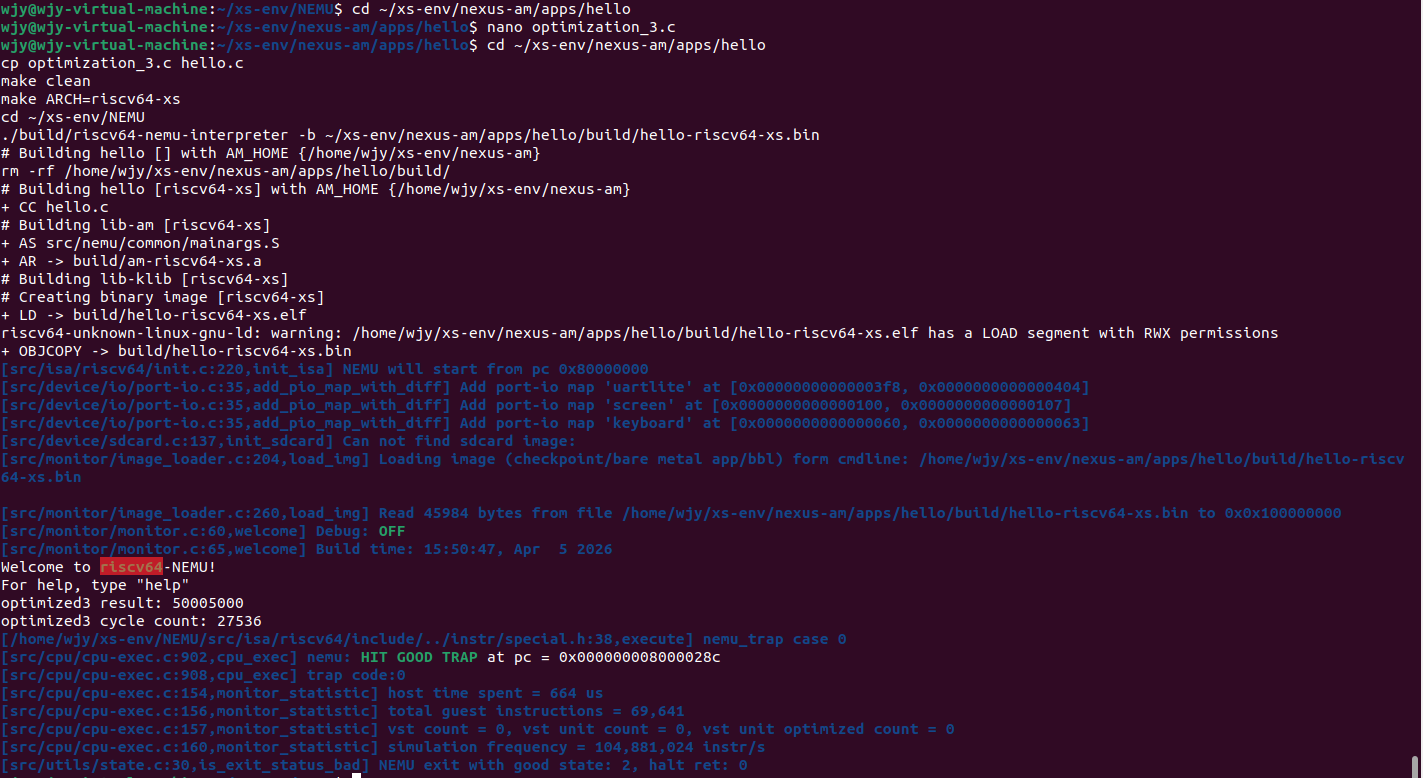
\includegraphics[width = 1\textwidth]{figure/three.png}
    \caption{任务二优化三运行结果截图}
\end{figure}
随后进一步实现优化四，在优化二思路上扩展为 8 路累加器与 8 路循环展开。该版本继续降低了循环控制开销和单一累加变量带来的顺序相关，使周期数进一步下降，最终成为本实验中性能最好的实现。
下面给出优化四运行结果截图，用于说明当前最佳版本在保持结果正确的前提下，已经获得了最低的周期数。

\begin{figure}[H]
    \centering
    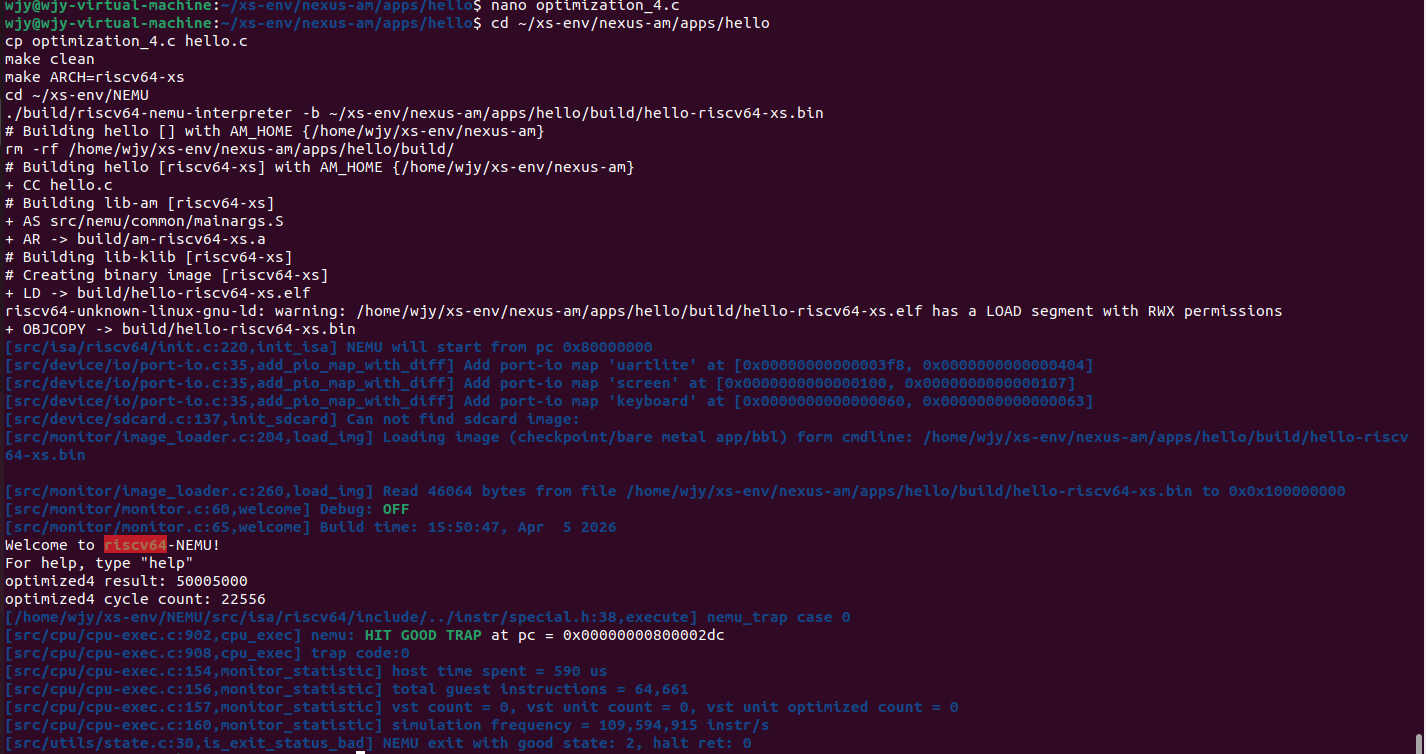
\includegraphics[width = 1\textwidth]{figure/four.png}
    \caption{任务二优化四运行结果截图}
\end{figure}

在完成四轮手工优化之后，为了进一步考察编译器优化的作用，又在不改变优化四算法结构的前提下，对核心函数增加了 \texttt{\_\_attribute\_\_((optimize("O3")))} 属性，尝试通过更高等级的编译器优化进一步压缩指令流并提升性能。实验结果表明，加入函数级 \texttt{O3} 后，程序输出结果仍然正确，但周期数与优化四相比未发生改变。这说明当前优化四代码本身已经较适合编译器自动优化，其结构已较接近当前实验环境下的高效实现形式，因此编译器优化在这一阶段未带来额外显著收益。

\begin{figure}[H]
    \centering
    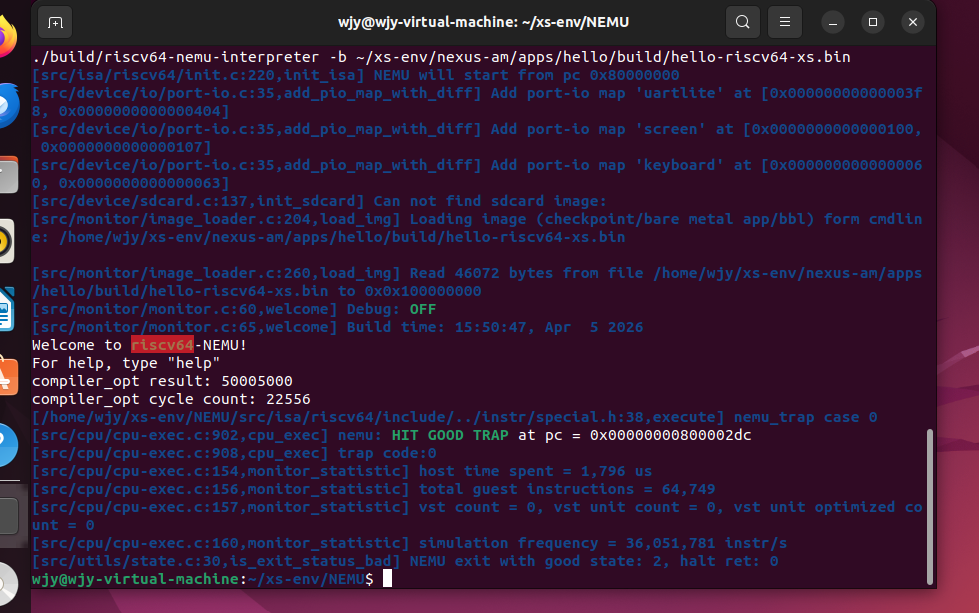
\includegraphics[width = 1\textwidth]{figure/O3.png}
    \caption{任务二编译器优化尝试结果截图}
\end{figure}

综合整个实验过程可以看出，本任务遵循了“先验证正确性，再逐步优化，再补充编译器优化分析”的推进顺序。基线版本用于建立参照标准；优化一至优化四用于考察减少过程调用、消除不必要存储引用、循环展开和多累加器设计等手工优化手段对性能的影响；编译器优化尝试则用于补充分析当前代码在更高优化等级下的表现。通过这样的实验过程设计，可以较清楚地观察不同优化方法对向量求和程序执行效率的影响。

\subsection{实验结果}
各版本程序在相同输入规模下运行后，均得到了正确的向量求和结果 \texttt{50005000}，说明优化过程没有破坏程序正确性。不同优化版本的周期数统计结果如表所示：

\begin{table}[H]
\centering
\caption{向量求和不同优化版本性能对比}
\begin{tabular}{llll}
\toprule
版本 & 优化方法 & 运行结果 & 周期数 \\
\midrule
基线版本 & 原始核心求和实现 & 50005000 & 50012 \\
优化一 & 直接数组访问 + 局部累加 & 50005000 & 40006 \\
优化二 & 4路循环展开 & 50005000 & 25032 \\
优化三 & 指针遍历 + 4路展开 & 50005000 & 27536 \\
优化四 & 8路累加器 + 8路展开 & 50005000 & 22556 \\
编译器优化尝试 & 优化四基础上增加函数级O3 & 50005000 & 22556 \\
\bottomrule
\end{tabular}
\end{table}

